\documentclass[fleqn,10pt]{physiome}
% Use option lineno for line numbers 
\usepackage{siunitx}
\usepackage{enumitem}  
\usepackage{subcaption}
\usepackage{graphicx}
\usepackage{lscape}
\articletype{Original}
%% Choose from Original, Retrospective, Review, Letter

\title{Reproducibility Study on a PBPK Model of FcRn-Mediated Recycling for Large Molecules}

\author[1][soroush.safaei@sanofi.com]{Soroush Safaei}
\author[1]{Veronique De Brabandere}
\author[3]{Wilhelmus E. A. de Witte}
\author[2]{Lindsay B. Avery}
\author[1]{Tom Van Bogaert}
\author[1]{Maria Laura Sargentini-Maier}
\affil[1]{Sanofi R\&D, Ghent, Belgium}
\affil[2]{Sanofi R\&D, Cambridge, USA}
\affil[3]{esqLABS GmbH, Saterland, Germany}

%% The following lines can be omitted when submitting;
%% information will be added by editors
\publicationdate{12 Feb 2024}
\editor{Shelley Fong}
\curator{Weiwei Ai}
\submitteddate{21 Nov 2023}
\accepteddate{08 Feb 2024}
\citethisas{Safaei et al. (2024)\\Reproducibility Study on a PBPK Model of FcRn-Mediated Recycling for Large Molecules. Physiome.}{10.36903/physiome.25194020}
\begin{document}

\maketitle

\begin{abstract}
The PBPK model of FcRn-mediated recycling of large molecules was developed and studied by \cite{de2023mechanistic} to characterize and predict Immunoglobulin G (IgG) disposition in plasma and tissues. This study investigated the large-molecule model in PK-Sim\textsuperscript{\textregistered} and its applicability to molecules with FcRn binding affinity in plasma. Subsequently, the model was extended to ensure a more mechanistic description of the internalization of FcRn and the FcRn-drug complex. This PBPK model has applications in autoimmune disorders such as primary immune thrombocytopenia which is mediated partly by platelet autoantibodies, resulting in thrombocytopenia, bleeding, and constitutional symptoms. Currently, there are several FcRn inhibitors in clinical development for numerous indications that can benefit from this model. We created a modular implementation of the model in MoBi\textsuperscript{\textregistered}\footnote{https://github.com/Open-Systems-Pharmacology/Suite/releases/tag/v11.2}, which is able to reproduce the originally published data. This Physiome paper describes how to access, run, and manipulate this model, how to parameterize the model to match data, and how to compare model predictions to data. In addition, some inconsistencies have been revealed and discussed in this paper.
\end{abstract}

\keywords{PBPK, FcRn, IgG, large molecules, monoclonal antibodies, PK-Sim\textsuperscript{\textregistered}, MoBi\textsuperscript{\textregistered}}

\primarypubs[10.36903/physiome.25194020]{sample}{de2023mechanistic}

%-------------------------------------------------------------------
%-------------------------------------------------------------------
%-------------------------------------------------------------------

\section{Introduction}

The pharmacokinetics of biologics, such as monoclonal antibodies (mAb), Fc-containing modalities, albumin fusions, and albumin binding constructs, are often significantly impacted by their binding to the FcRn receptor. These molecules have very little affinity to the FcRn receptor on the cell membranes of endothelial and hematopoietic cells in the plasma space at the physiological plasma pH, but have an affinity of approximately $1$ \si{\micro M} at a lower endosomal pH. The binding of wild-type IgGs and Albumin constructs to FcRn at neutral pH in plasma is weak. However, a growing number of Fc-engineered constructs have been developed to improve pharmacokinetics, FcRn inhibition, or FcRn-mediated target sweeping, and these have been shown to have enhanced binding at plasma pH. 

In PBPK models for large molecules, FcRn binding is often explicitly described, but usually only in the endosomal space. The original PK-Sim\textsuperscript{\textregistered} model for large molecules, as described by \cite{niederalt2018generic}, includes binding to FcRn in both the plasma and endosomal space, and also takes into account endogenous IgG and its binding to FcRn to account for competition between mAbs and endogenous IgG. However, the model does not include internalization of the FcRn-drug complex, and therefore cannot describe a decreasing half-life with increasing FcRn binding affinity in plasma. In the primary article, \cite{de2023mechanistic} investigated the FcRn binding part of the large-molecule model in PK-Sim\textsuperscript{\textregistered}, evaluated its applicability to molecules with enhanced FcRn binding at plasma pH, and further extended the model in MoBi\textsuperscript{\textregistered} for FcRn inhibitors.

Here, we presented a modular implementation of the MoBi\textsuperscript{\textregistered} model developed by \cite{de2023mechanistic} which successfully reproduced all simulation results in the primary paper, allows future studies to import other molecules or administration protocols. In this model, the internalization and recycling of FcRn and the FcRn-drug complex are explicitly incorporated which makes the PK/PD prediction of FcRn inhibitors with increased plasma and endosomal affinities in different species possible. These improvements allow investigations of IgG tissue distribution, and prediction of antibody biodistribution. The model can guide preclinical evaluations of FcRn inhibitors in development, potentially helping with dose optimization strategies for this emerging class of immunosuppressive drugs. 

%-------------------------------------------------------------------
%-------------------------------------------------------------------
%-------------------------------------------------------------------

\section{Model Description}

Throughout this paper, the original PK-Sim\textsuperscript{\textregistered} model is referred to as the ``Net Model'', and the developed model as the ``Extended Model''. To modify the net model, the default mice PK-Sim\textsuperscript{\textregistered} model was first built 
 in PK-Sim\textsuperscript{\textregistered} and exported to MoBi\textsuperscript{\textregistered}. This base model can be found at \url{https://models.physiomeproject.org/workspace/b37}. We attempted to make minimal changes to the existing model structure in MoBi\textsuperscript{\textregistered} and reused some existing parameters for a new purpose. In PK-Sim\textsuperscript{\textregistered}, \textit{K\_rec} and \textit{K\_uptake} are the parameter names for the parameters indicated by \textit{k\_recnetComp} and \textit{k\_intnetFcRn} in the manuscript. In the extended model, the original net model parameter names can be kept as \textit{K\_rec} and \textit{K\_uptake} in their original equations, but now they represent \textit{k\_rec} and \textit{k\_int} as these equations will be applied to both free and bound FcRn. In the following, all the steps for reparameterization are described and illustrated with MoBi\textsuperscript{\textregistered} screenshots.


\subsection{Adding FcRn complexes internalization}\label{SS1}

\begin{enumerate}[label=(\roman*)]
    \item {Find the transport that internalizes the free FcRn to the endosome:}
    \begin{itemize}
        \item \textit{NetMassTransfer\_PlasmaToEndosomal\_FcRn}
    \end{itemize}
    \item {Add the relevant FcRn complexes to this transport:} \\
In order to take into account the internalization of free FcRn, IgG-bound FcRn and drug-bound FcRn, they can be included in the "Passive Transports" building block. Add the following molecules to the "Include List" field.
    \begin{itemize}
        \item \textit{LigandEndo\_Complex}
        \item \textit{Drug-FcRn\_Complex}
    \end{itemize}
    \item{Make sure the tags apply to the new complexes:} \\
To ensure that internalizations occur in all endosomes, the ``Endogenous\_IgG'' tag should be taken away from the source and target fields. This will make the process effective, as demonstrated in Figure~\ref{pic1}\subref{pic:1a}.
    \begin{itemize}
        \item \textit{Endogenous\_IgG}
    \end{itemize}
	\item{Make sure the parameter paths are applicable to the new complexes:}\\
The ``f\_membrane\_pls'' parameter is not found in the tissue endosomes, so the path to it must be altered in the ``Kinetic'' tab of the transport. To do this, an absolute path has been set, as illustrated in Figure~\ref{pic1}\subref{pic:1b}.
    \begin{itemize}
        \item \textit{Organism|EndogenousIgG|f\_membrane\_pls}
    \end{itemize}
\end{enumerate}

\begin{figure}[htb]\centering
    \begin{subfigure}{0.49\textwidth}
        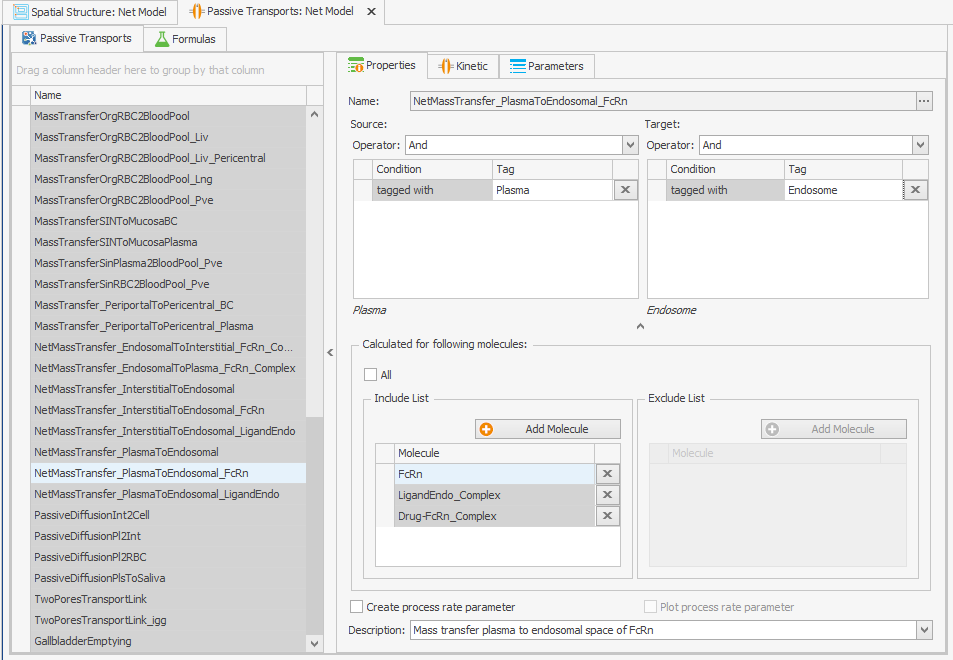
\includegraphics[width=\textwidth]{Picture2.png}
        \caption{}
        \label{pic:1a}
    \end{subfigure}
    \hfill
    \begin{subfigure}{0.49\textwidth}
        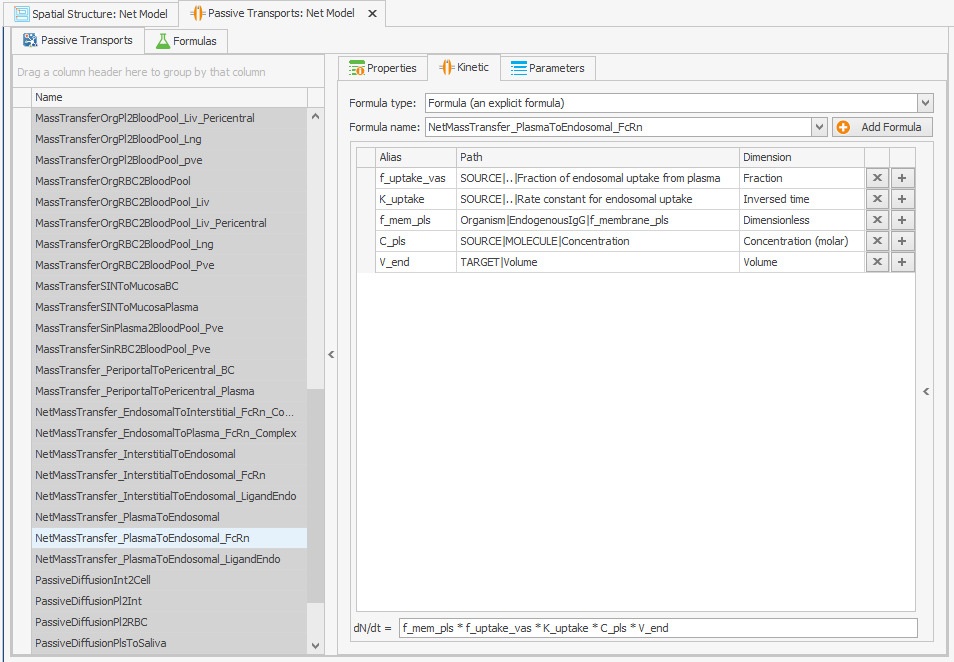
\includegraphics[width=\textwidth]{Picture3.png}
        \caption{}
        \label{pic:1b}
    \end{subfigure}
    \caption{Screenshots of (a) the modified setup of plasma to endosomal FcRn and FcRn complexes internalization and (b) the modified reference path in the reparametrized model.}
    \label{pic1}
\end{figure}


\subsection{Adding free FcRn recycling}

\begin{enumerate}[label=(\roman*)]
    \item {Find the transport that recycles the FcRn complexes:}
    \begin{itemize}
        \item \textit{NetMassTransfer\_EndosomalToPlasma\_FcRn\_Complex}
    \end{itemize}
    \item {Add the free FcRn to this transport:} \\
Incorporating recycling of free FcRn into the model can be achieved by adding it as a molecule to the "Passive Transport" from endosome to plasma as depicted in Figure~\ref{pic2}. No alterations to the transport kinetics are necessary.
    \begin{itemize}
        \item \textit{FcRn}
    \end{itemize}
\end{enumerate}

\begin{figure}[htb]\centering
    \begin{subfigure}{0.49\textwidth}
        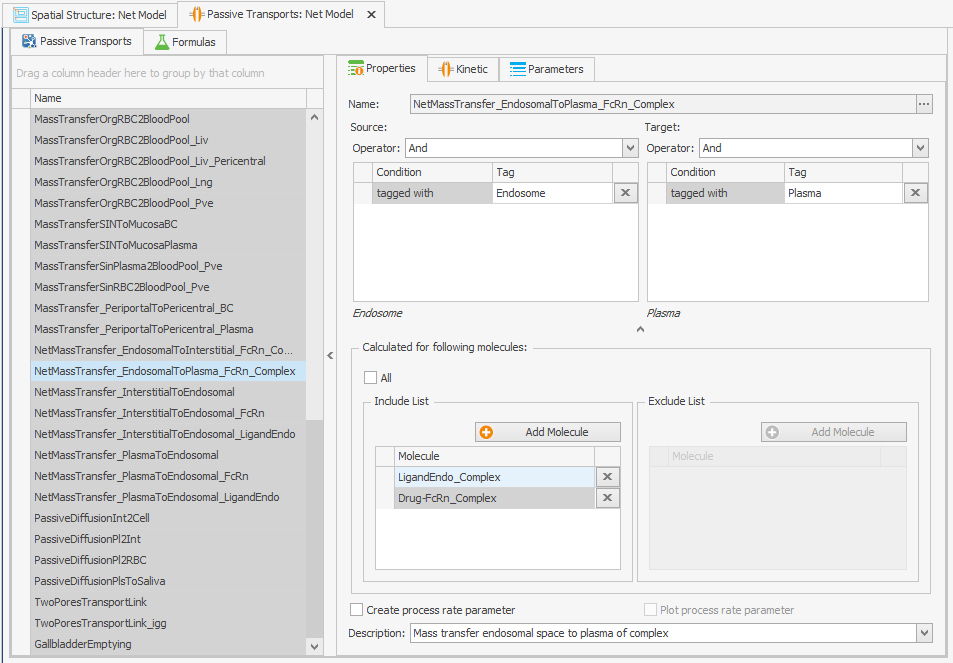
\includegraphics[width=\textwidth]{Picture4.png}
        \caption{}
        \label{pic:2a}
    \end{subfigure}
    \hfill
    \begin{subfigure}{0.49\textwidth}
        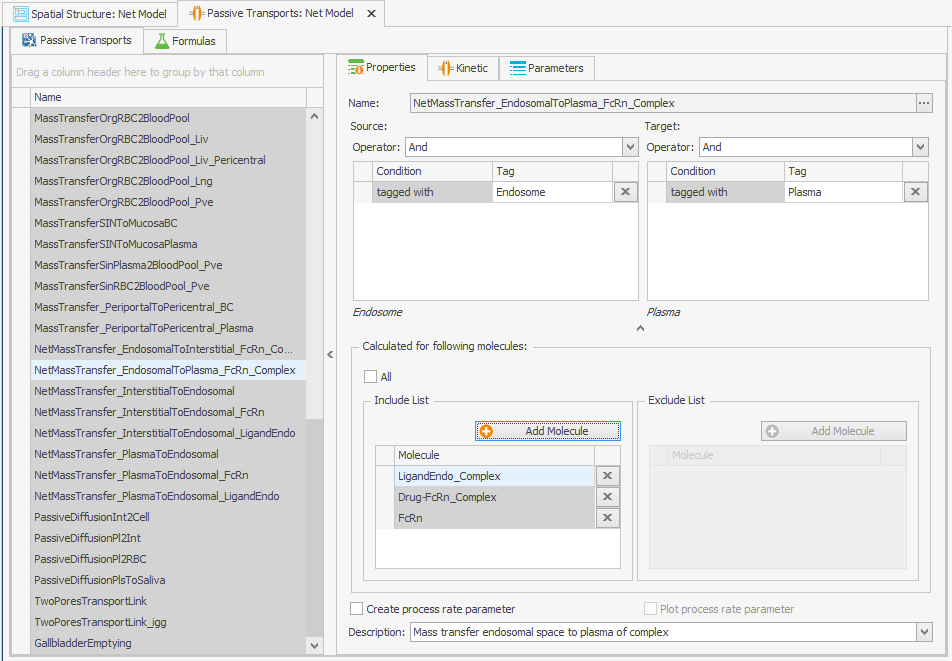
\includegraphics[width=\textwidth]{Picture5.png}
        \caption{}
        \label{pic:2b}
    \end{subfigure}
    \caption{Screenshots of (a) the original and (b) the modified setup of the endosomal to plasma FcRn and FcRn complexes recycling.}
    \label{pic2}
\end{figure}



\subsection{Changing parameter values}

In order to ensure that the same model behavior is maintained for typical IgGs, the parameter values must be altered as outlined in the original article. The most significant change that needs to be made is to modify the ``Rate constant for endosomal uptake (global)'' (i.e., \textit{K\_uptake}) from $0.294$ to $0.494$/min. This should be done directly at the organism level in the ``Spatial Structures'' building block to guarantee that the global parameter value is modified as depicted in Figure~\ref{pic4}\subref{pic:4a} (there is a parameter with the same name at the endogenous IgG level, but this takes the value of the global parameter).

\begin{itemize}
    \item \textit{Organism|Rate constant for endosomal uptake (global):} $0.294$ --> $0.494$/min
\end{itemize}

The ``Specific clearance (endosome)'' parameter is initially determined by subtracting the net FcRn internalization rate constant from the net FcRn complex recycling rate constant. The source of this calculation is not explicitly stated in \cite{niederalt2018generic}, so we kept the original model behavior by changing the equation to a value of $0.205$/min in the ``Spatial Structures'' building block, as illustrated in Figure~\ref{pic4}\subref{pic:4b}.
	
\begin{itemize}
    \item \textit{Organism|Specific clearance (endosome):} K\_uptake-K\_rec>=0 ? K\_uptake-K\_rec : 0 \\
    --> $0.205$/min
\end{itemize}

To guarantee that the steady-state calculation for the determination of initial molecule concentrations is done with the right parameter values, the formula for calculating \textit{IgG\_kpe} and \textit{krpls} in the ``Spatial Structures'' building block was modified by substituting \textit{K\_uptake} with its original value, as illustrated in Figure~\ref{pic4}\subref{pic:4c} and~\ref{pic4}\subref{pic:4d}.

\begin{itemize}
    \item \textit{Organism|EndogenousIgG|IgG\_kpe:} f\_uptake\_vas*K\_uptake*V\_end \\ --> f\_uptake\_vas*0.294*V\_end
    \item \textit{Organism|EndogenousIgG|krpls:} f\_mem\_pls*f\_uptake\_vas*K\_uptake*V\_end \\--> f\_mem\_pls*f\_uptake\_vas*0.294*V\_end
\end{itemize}

At this stage, the most straightforward way to achieve the desired outcome is to substitute \textit{K\_uptake} with its original value. This could be altered in the future to include the pertinent parameter.

\begin{figure}[htb]\centering
    \begin{subfigure}{0.49\textwidth}
        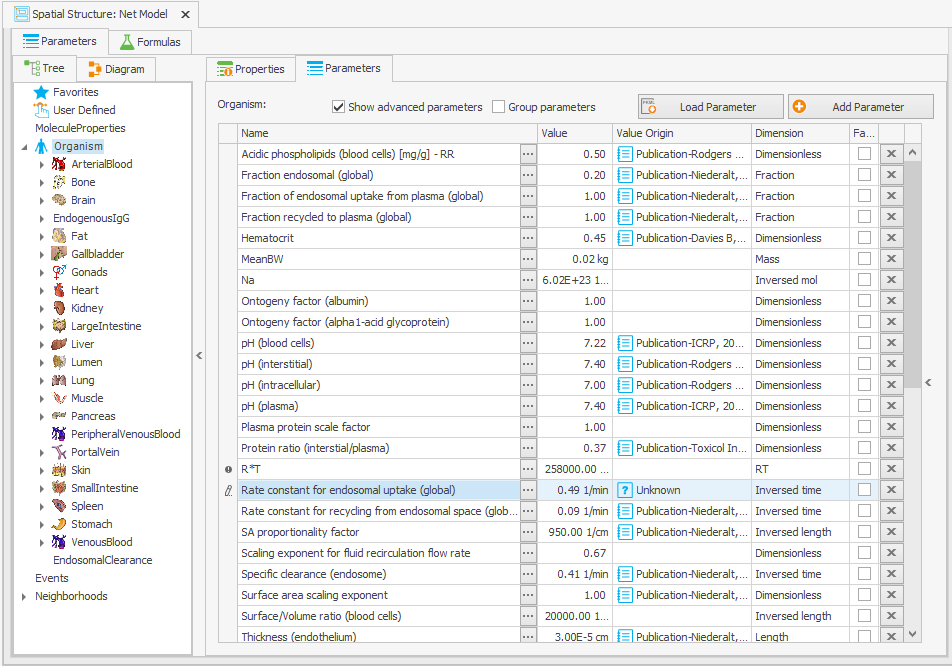
\includegraphics[width=\textwidth]{Picture8.png}
        \caption{}
        \label{pic:4a}
    \end{subfigure}
    \hfill
    \begin{subfigure}{0.49\textwidth}
        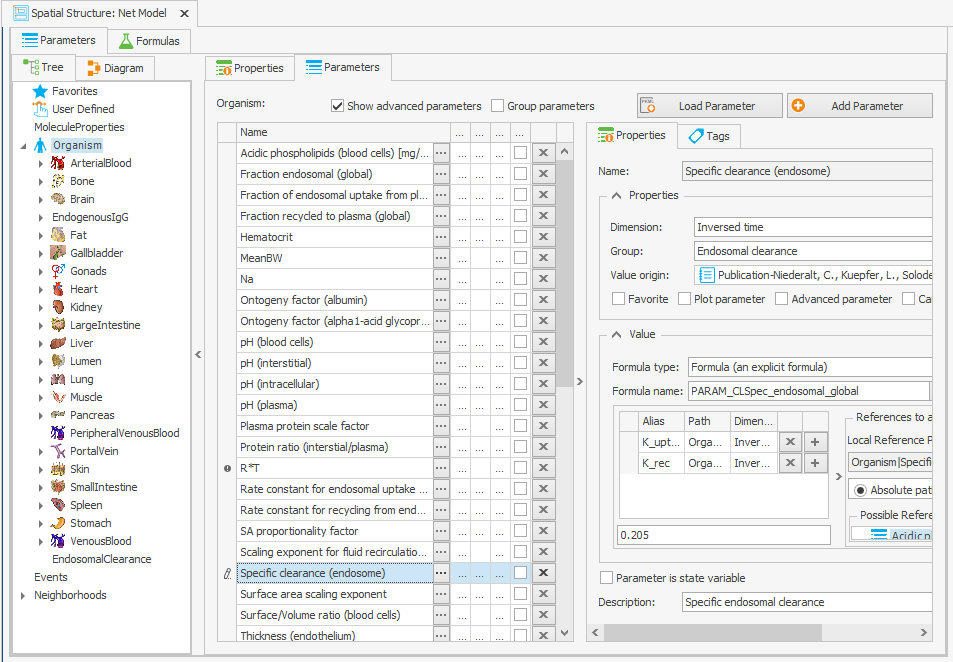
\includegraphics[width=\textwidth]{Picture9.png}
        \caption{}
        \label{pic:4b}
    \end{subfigure}
    \hfill
    \begin{subfigure}{0.49\textwidth}
        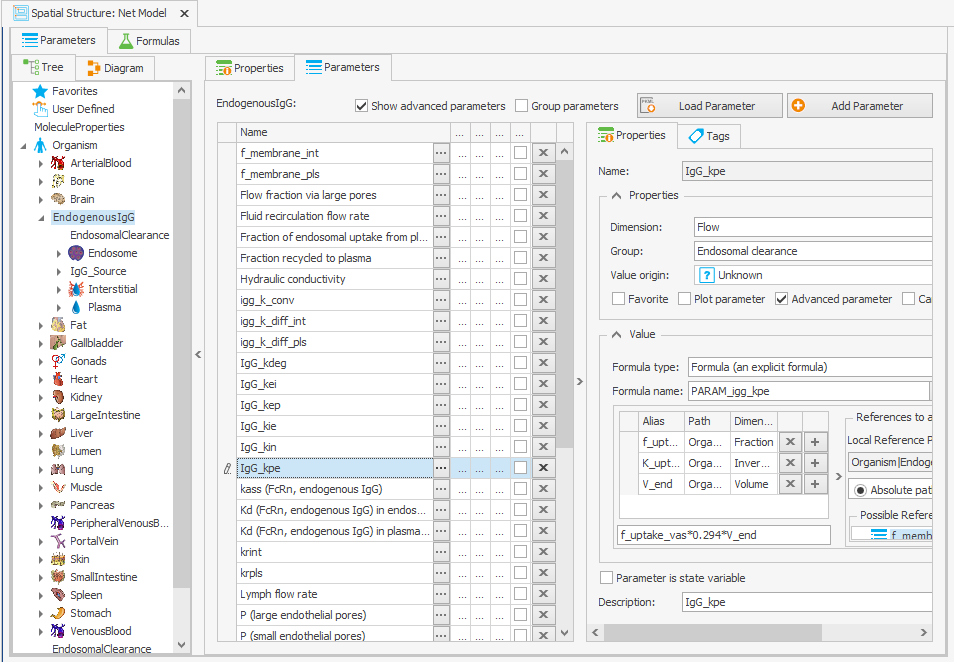
\includegraphics[width=\textwidth]{Picture10.png}
        \caption{}
        \label{pic:4c}
    \end{subfigure}
    \hfill
    \begin{subfigure}{0.49\textwidth}
        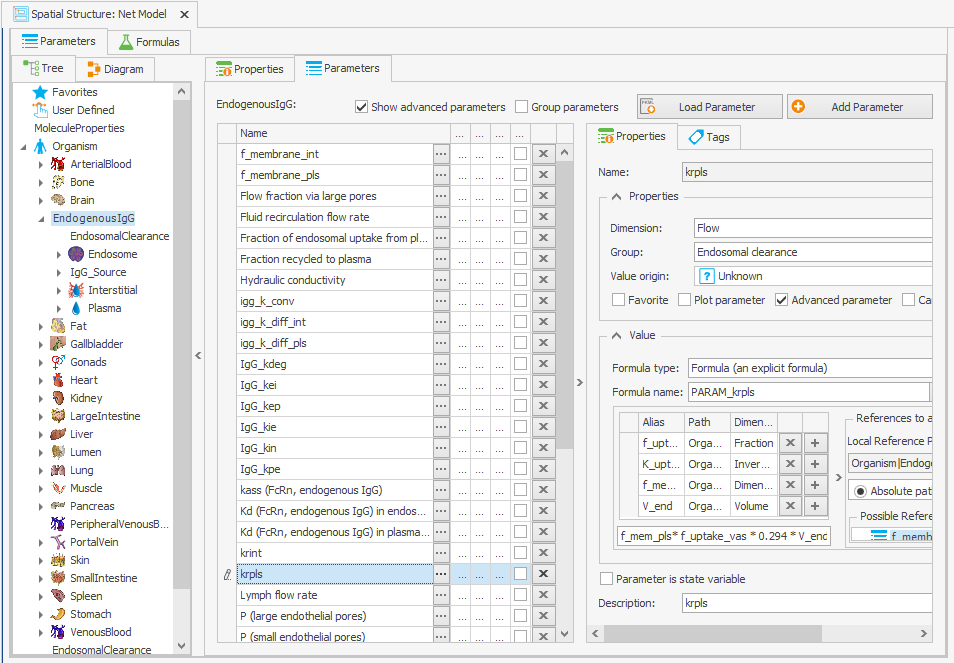
\includegraphics[width=\textwidth]{Picture11.png}
        \caption{}
        \label{pic:4d}
    \end{subfigure}
    \caption{Screenshot of the modified setup for (a) Rate constant for endosomal uptake (global) and (b) Specific clearance (endosome). Screenshots of the modified equation for (c) IgG\_kpe and (d) krpls.}
    \label{pic4}
\end{figure}



\subsection{Reduce internalization of unbound protein}

The internalization rate constants of the unbound protein and the FcRn-bound protein are linked through the volume ratios of the endosome and plasma. In the original model, this volume ratio is applied to the net mass transfer of free FcRn, rather than to its internalization. In the reparameterized model, this volume ratio is instead applied to the internalization rate constants, which leads to an increase in the uptake of unbound protein, as the internalization rate constant is higher than the net mass transfer. Since the uptake parameter of unbound protein in the model was calibrated on a large dataset, including data from FcRn knockout mice, this increase in the uptake of unbound protein needs to be adjusted in the reparameterized model. The \textit{k\_int} value is calculated as $0.494$ while the \textit{k\_intnetFcRn} was $0.294$, so this can be corrected by multiplying the internalization transport of the unbound protein by $0.294/0.494=0.595$. This must also be done for the endogenous ligand, as shown in Figures~\ref{pic3}.

\begin{itemize}
    \item \textit{NetMassTransfer\_PlasmaToEndosomal}
    \item \textit{NetMassTransfer\_PlasmaToEndosomal\_LigandEndo}
\end{itemize}

\begin{figure}[htb]\centering
    \begin{subfigure}{0.49\textwidth}
        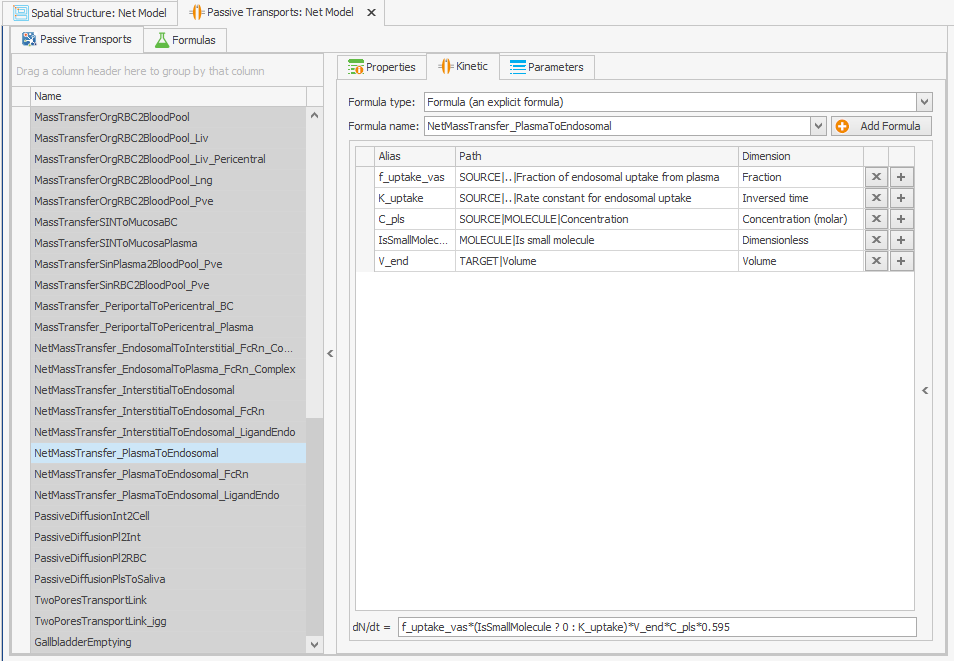
\includegraphics[width=\textwidth]{Picture6.png}
        \caption{}
        \label{pic:3a}
    \end{subfigure}
    \hfill
    \begin{subfigure}{0.49\textwidth}
        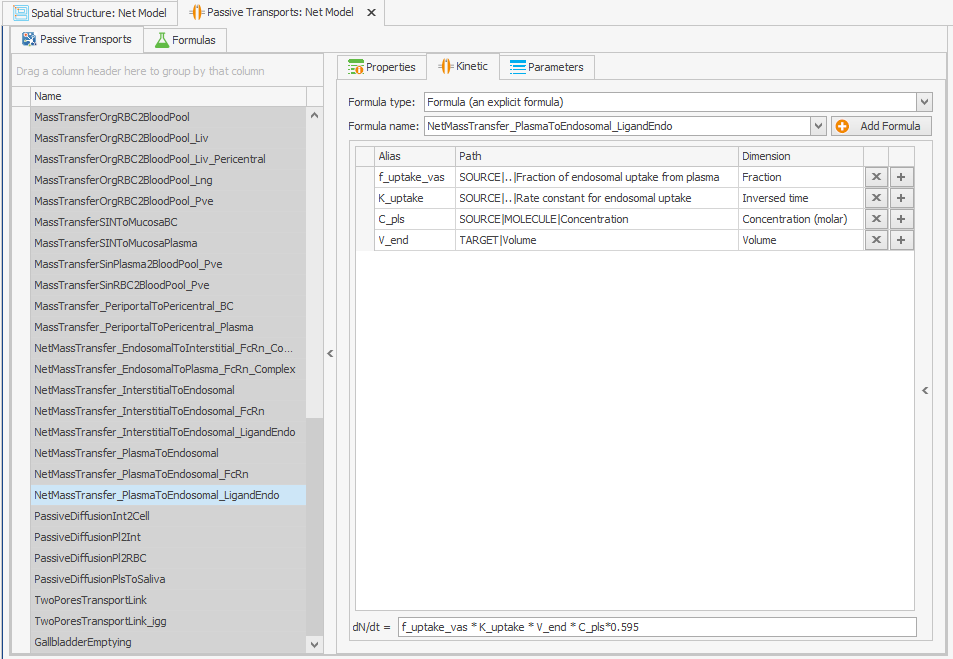
\includegraphics[width=\textwidth]{Picture7.png}
        \caption{}
        \label{pic:3b}
    \end{subfigure}
    \caption{Screenshot of (a) the modified equation in the kinetic tab of the plasma to endosomal transport for unbound protein (b) and endogenous ligand.}
    \label{pic3}
\end{figure}


\subsection{Extending and checking the parameters starting values}

Press "Extend" to update the parameter starting values building block. Select the parameter ``Rate constant for endosomal uptake (global)'' to update parameters that have changed values in the building block. Click "Apply" next to "Refresh all from source".



\subsection{Modifications (WT Mice -> Tg32 Mice)}\label{MC}

We adjusted the endogenous IgG affinity in endosome to a very low value of $1$ M, instead of the default $0.75$ \si{\micro M}, to reflect the lack of binding of endogenous IgG in mice to human FcRn in Tg32 mice. This also applied to the endogenous IgG affinity in plasma.

\begin{itemize}
    \item \textit{Drug|Kd (FcRn, endogenous IgG) in endosomal space:} $0.75$ \si{\micro M} -> $1$ \si{M}
    \item \textit{Drug|Kd (FcRn, endogenous IgG) in plasma space:} $10000$ \si{\micro M} -> $1$ \si{M}
\end{itemize}

\begin{table}[htbp]
\centering
    \begin{threeparttable}
        \caption{Simulated amounts and concentrations of FcRn molecular species in the net model at steady state.}\label{tbl:1}
        \begin{tabular}{llcc}
            \toprule
            Molecule & Location & Amount (\si{\micro mol}) & Concentration (\si{\micro M}) \\
            \midrule
            FcRn:EndoIgG & Endosome & $29.0\times10^{-5}$ & $56.7$ \\
            FcRn & Endosome & $19.8\times10^{-5}$ & $38.7$ \\
            FcRn & Plasma & $8.75\times10^{-5}$ & $0.177$ \\
            \bottomrule
        \end{tabular}
    \end{threeparttable}
\end{table}

In order to account for the free endosomal FcRn concentration, it was necessary to adjust the total FcRn concentration in WT and Tg32 mice, which was assumed to be the same based on limited literature data. To calculate the total endosomal FcRn, we added the free and endogenous IgG-bound FcRn concentrations in the endosome at steady state in the net model (from Table~\ref{tbl:1}), resulting in a new parameter value of $95.4$ \si{\micro M} instead of the original $38.7$ \si{\micro M}.

\begin{itemize}
    \item \textit{Organism|EndogenousIgG|Endosome|Start concentration of free FcRn (endosome):} $95.4$ \si{\micro M}
\end{itemize}

We have identified a mistake in the original article concerning the free endosomal FcRn concentration, which is actually $95.4$ \si{\micro M} instead of the previously reported $92.5$ \si{\micro M}. Nevertheless, the simulation results in the original article are based on the accurate parameter value. The precise concentration values for FcRn molecular species are provided in Table~\ref{tbl:1}.

%-------------------------------------------------------------------
%-------------------------------------------------------------------
%-------------------------------------------------------------------

\section{Model Execution}

The results were created using MoBi\textsuperscript{\textregistered} Version $11$. The model simulation file can be found at \url{https://models.physiomeproject.org/workspace/b37}. The file includes three models, which are identified by the simulation names in the file. To generate results, follow the step-by-step instructions for each figure.


\subsection{Net Model for WT Mice (figure 2 in primary article)}\label{Figure2}

The initial simulation examined a standard mAb molecule in mice without FcRn binding in the plasma (with an affinity of 1 M) and an endosomal FcRn affinity of 1 µM. This simulation tracked the mAb concentration in the plasma, the amount of free FcRn in the plasma, free FcRn in the endosome, and the FcRn bound to endogenous IgG over time for doses of $1$ and $100$ mg/kg.

\subsubsection{Load the model}
Open the ``Physiome.mbp3'' file using MoBi\textsuperscript{\textregistered} and in ``Simulations'' explorer double-click on ``\textit{Net Model}'' entry.

\subsubsection{Set the Simulation for 1 mg/kg}
\begin{itemize}
    \item In the ``Parameters'' tab of our simulation, click on ``Favorites''.
    \item Change the value of the parameter: 
    \begin{itemize}
        \item \textit{DosePerBodyWeight} --> $1$ mg/kg.
    \end{itemize}
    \item ``Run'' the simulation.
    \item Rename the result in the ``Simulations'' explorer under the ``\textit{Net Model}'' entry to ``$1$ mg/kg''.
\end{itemize}

\subsubsection{Set the Simulation for 100 mg/kg}
Rather than creating a new simulation for each instance, we will simply adjust the dose in the existing one.
\begin{itemize}
    \item In the ``Parameters'' tab of our simulation, click on ``Favorites''.
    \item Change the value of the parameter: 
    \begin{itemize}
        \item \textit{DosePerBodyWeight} --> $100$ mg/kg.
    \end{itemize}
    \item ``Run'' the simulation.
    \item Rename the result in the ``Simulations'' explorer under the ``\textit{Net Model}'' entry to ``$100$ mg/kg''.
\end{itemize}

\subsubsection{Compare the Results}
\begin{itemize}
    \item Double-click ``$100$ mg/kg'' in the simulation results.
    \item Drag \& drop ``$1$ mg/kg'' result onto the plot (We make it visible later).
    \item In the ``Chart Editor'', select only the ``Drug'' simulations.
    \item Make sure the Y-axis scaling is ``Log'' in the tab ``Curves and Axis Options''.
    \item Change the ``Curve Name'' in the tab "Curves and Axis Options''.
    \begin{itemize}
        \item \textit{100 mg/kg-Organism-PeripheralVenousBlood-Drug-Plasma (Peripheral Venous Blood)} 
        \\--> Dose 100 mg/kg
        \item \textit{1 mg/kg-Organism-PeripheralVenousBlood-Drug-Plasma (Peripheral Venous Blood)} 
        \\--> Dose 1 mg/kg
    \end{itemize}
    \item Adjust the colors and change the title and legend position in the tab ``Chart Options''.
    \item You can find the results in Figure~\ref{fig:1}\subref{fig:1a}.
    \item Double-click ``$100$ mg/kg'' in the simulation results again.
    \item Drag \& drop ``$1$ mg/kg'' result onto the plot (We make it visible later).
    \item In the ``Chart Editor'', select only the ``FcRn'' and ``LigandEndo\_Complex'' simulations.
    \item Make sure the Y-axis scaling is ``Linear'' in the tab ``Curves and Axis Options''.
    \item Change the ``Curve Name'' in the tab "Curves and Axis Options''.
    \begin{itemize}
        \item \textit{100 mg/kg-Organism-EndogenousIgG-Endosome-FcRn-Amount in container} 
        \\--> FcRn in Endosome - 100 mg/kg
        \item \textit{100 mg/kg-Organism-EndogenousIgG-Plasma-FcRn-Amount in container} 
        \\--> FcRn in Plasma - 100 mg/kg
        \item \textit{1 mg/kg-Organism-EndogenousIgG-Endosome-FcRn-Amount in container} 
        \\--> FcRn in Endosome - 1 mg/kg
        \item \textit{1 mg/kg-Organism-EndogenousIgG-Plasma-FcRn-Amount in container} 
        \\--> FcRn in Plasma - 1 mg/kg
        \item \textit{1 mg/kg-Organism-EndogenousIgG-Endosome-LigandEndo\_Complex-Amount in container} --> FcRn:IgG in Endosome - 1 mg/kg
        \item \textit{100 mg/kg-Organism-EndogenousIgG-Endosome-LigandEndo\_Complex-Amount in container} --> FcRn:IgG in Endosome - 100 mg/kg
    \end{itemize}
    \item Adjust the colors and change the title and legend position in the tab ``Chart Options''.
    \item You can find the results in Figure~\ref{fig:1}\subref{fig:1b}.
\end{itemize}

\begin{figure}[htb]\centering
    \begin{subfigure}{0.49\textwidth}
        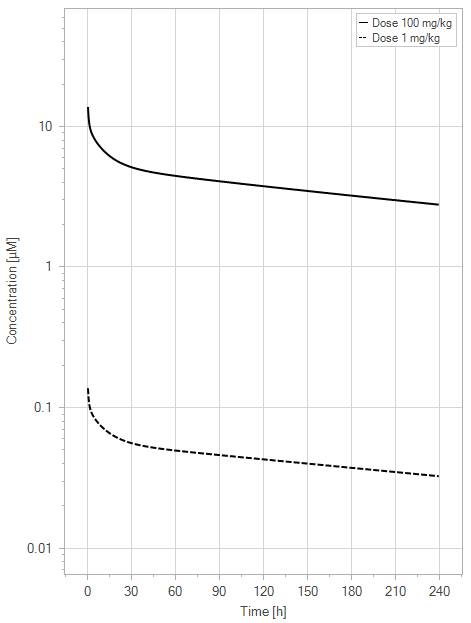
\includegraphics[width=\textwidth]{pl1.png}
        \caption{PK profiles}
        \label{fig:1a}
    \end{subfigure}
    \hfill
    \begin{subfigure}{0.49\textwidth}
        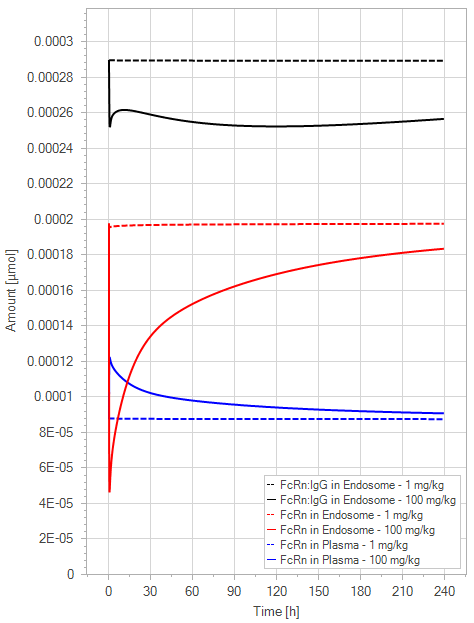
\includegraphics[width=\textwidth]{pl2.png}
        \caption{PD Profiles}
        \label{fig:1b}
    \end{subfigure}
    \caption{The ``\textit{Net Model}'' response for a typical antibody (not binding to FcRn in plasma with $1$ \si{M} affinity, binding in endosome with $1$ \si{\micro M} affinity) with two different doses ($1$ and $100$ mg/kg). (a) Lines correspond to drug plasma concentrations. (b) Lines corresponds to free FcRn amounts in plasma (blue), free FcRn amounts in endosome (red) and FcRn:endogenous IgG complexes amounts in endosome (black). This figure corresponds to figure 2 in the primary article.}
    \label{fig:1}
\end{figure}



\subsection{Net Model for WT Mice (figure 3 in primary article)}\label{Figure3}

The second simulation was conducted to determine the impact of the mAb concentration in the default mice model in relation to the FcRn binding affinity. This was done by altering the plasma FcRn binding affinity of the mAb from no binding ($1$ M) to high affinity binding ($1$ nM) for a dose of $1$ mg/kg with $1000$-fold steps, while the endosomal FcRn affinity remained constant at $1$ \si{\micro M}.

\begin{figure}[htb]\centering
    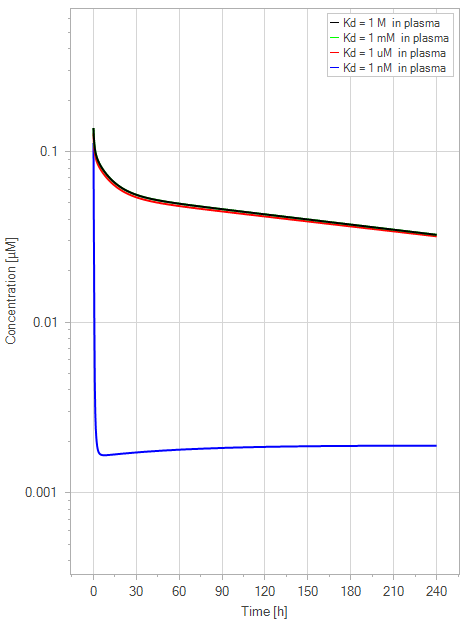
\includegraphics[width=0.49\linewidth]{pl3}
    \caption{The ``\textit{Net Model}'' response for FcRn binding antibodies. The different line colors correspond to different FcRn affinities in plasma. All lines are overlapping except the $1$ nM (blue) affinity line. The endosomal FcRn affinity and all other parameters are kept constant at the default parameters as in Figure~\ref{fig:1} with a dose of $1$ mg/kg. This figure corresponds to figure 3 in the primary article.}
    \label{fig:2}
\end{figure}

\subsubsection{Load the model}
Open the ``Physiome.mbp3'' file using MoBi\textsuperscript{\textregistered} and in ``Simulations'' explorer double-click on ``\textit{Net Model}'' entry.

\subsubsection{Set the Simulation for 1 nM}
\begin{itemize}
    \item In the ``Parameters'' tab of our simulation, click on ``Favorites''.
    \item Change the value of the parameter: 
    \begin{itemize}
        \item \textit{DosePerBodyWeight} --> $1$ mg/kg.
        \item \textit{Kd (FcRn) in plasma/interstitial} --> $1$ nM
    \end{itemize}
    \item ``Run'' the simulation.
    \item Rename the result in the ``Simulations'' explorer under the ``\textit{Net Model}'' entry to ``Kd = $1$ nM''.
\end{itemize}

\subsubsection{Set the Simulation for 1 \si{\micro M}}
\begin{itemize}
    \item In the ``Parameters'' tab of our simulation, click on ``Favorites''.
    \begin{itemize}
        \item \textit{Kd (FcRn) in plasma/interstitial} --> $1$ \si{\micro M}
    \end{itemize}
    \item ``Run'' the simulation.
    \item Rename the result in the ``Simulations'' explorer under the ``\textit{Net Model}'' entry to ``Kd = $1$ \si{\micro M}''.
\end{itemize}

\subsubsection{Set the Simulation for 1 mM}
\begin{itemize}
    \item In the ``Parameters'' tab of our simulation, click on ``Favorites''.
    \begin{itemize}
        \item \textit{Kd (FcRn) in plasma/interstitial} --> $1$ mM
    \end{itemize}
    \item ``Run'' the simulation.
    \item Rename the result in the ``Simulations'' explorer under the ``\textit{Net Model}'' entry to ``Kd = $1$ mM''.
\end{itemize}

\subsubsection{Set the Simulation for 1 M}
\begin{itemize}
    \item In the ``Parameters'' tab of our simulation, click on ``Favorites''.
    \begin{itemize}
        \item \textit{Kd (FcRn) in plasma/interstitial} --> $1$ M
    \end{itemize}
    \item ``Run'' the simulation.
    \item Rename the result in the ``Simulations'' explorer under the ``\textit{Net Model}'' entry to ``Kd = $1$ M''.
\end{itemize}

\subsubsection{Compare Results}
\begin{itemize}
    \item Double-click ``Kd = $1$ M'' in the simulation results.
    \item Drag \& drop ``Kd = $1$ mM'' result onto the plot (We make it visible later).
    \item Drag \& drop ``Kd = $1$ \si{\micro M}'' result onto the plot (We make it visible later).
    \item Drag \& drop ``Kd = $1$ nM'' result onto the plot (We make it visible later).
    \item In the ``Chart Editor'', select only the ``Drug'' simulations.
    \item Make sure the Y axis scaling is ``Log'' in the tab ``Curves and Axis Options''.
    \item Change the ``Curve Name'' in the tab "Curves and Axis Options''.
    \begin{itemize}
        \item \textit{Kd = 1 M-Organism-PeripheralVenousBlood-Drug-Plasma (Peripheral Venous Blood)} 
        \\--> Kd = 1 M in plasma
        \item \textit{Kd = 1 mM-Organism-PeripheralVenousBlood-Drug-Plasma (Peripheral Venous Blood)} 
        \\--> Kd = 1 mM in plasma
        \item \textit{Kd = 1 uM-Organism-PeripheralVenousBlood-Drug-Plasma (Peripheral Venous Blood)} 
        \\--> Kd = 1 uM in plasma
        \item \textit{Kd = 1 nM-Organism-PeripheralVenousBlood-Drug-Plasma (Peripheral Venous Blood)} 
        \\--> Kd = 1 nM in plasma
    \end{itemize}
    \item Adjust the colors and change the title and legend position in the tab ``Chart Options''.
    \item You can find the results in Figure~\ref{fig:2}.
\end{itemize}



\subsection{Extended Model for WT Mice (figure 4 in primary article)}\label{Figure4}

To explore the difference in the performance of the extended model compared to the net model, the simulation in Figure~\ref{fig:1} was repeated with the extended model, yielding the results in Figure~\ref{fig:3}.

\subsubsection{Load the model}
Open the ``Physiome.mbp3'' file using MoBi\textsuperscript{\textregistered} and double-click on the ``Extended Model'' entry in the ``Simulations'' explorer. The steps that follow are the same as those described in Section~\ref{Figure2}, and the results can be seen in Figure~\ref{fig:3}.

\begin{figure}[htb]\centering
    \begin{subfigure}{0.49\textwidth}
        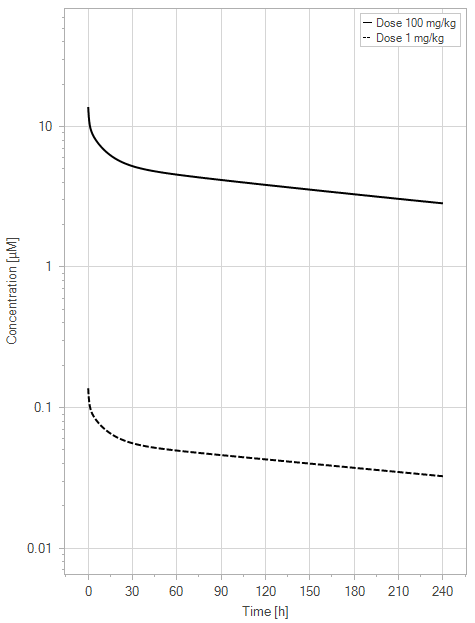
\includegraphics[width=\textwidth]{pl4.png}
        \caption{PK profiles}
        \label{fig:3a}
    \end{subfigure}
    \hfill
    \begin{subfigure}{0.49\textwidth}
        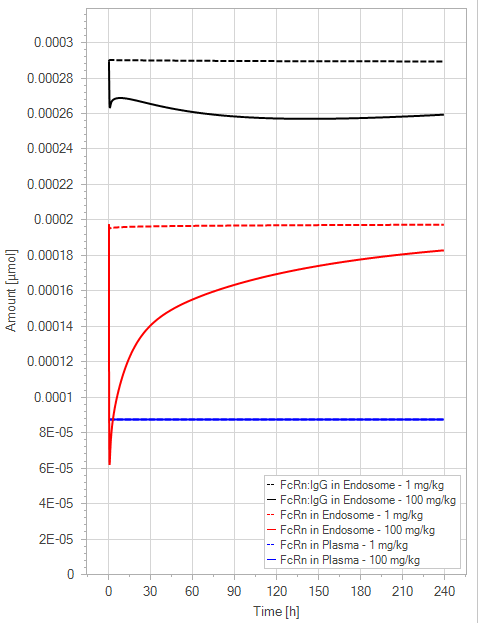
\includegraphics[width=\textwidth]{pl5.png}
        \caption{PD Profiles}
        \label{fig:3b}
    \end{subfigure}
    \caption{The ``\textit{Extended Model}'' response for a typical antibody (not binding to FcRn in plasma with $1$ \si{M} affinity, binding in endosome with $1$ \si{\micro M} affinity) with two different doses ($1$ and $100$ mg/kg). (a) Lines correspond to drug plasma concentrations. (b) Lines corresponds to free FcRn amounts in plasma (blue), free FcRn amounts in endosome (red) and FcRn:endogenous IgG complexes amounts in endosome (black). This figure corresponds to figure 4 in the primary article.}
    \label{fig:3}
\end{figure}

We have identified a minor issue in the legend for Figure 4 in the main article. The solid line corresponds to the $100$ mg/kg dose and the dashed line to the $1$ mg/kg dose.



\subsection{Extended Model for WT Mice (figure 5 in primary article)}\label{Figure5}

A second simulation was conducted using the extended model to assess the desired rise in the plasma half-life sensitivity of mAb to the FcRn binding affinity in plasma. This was done in the same way as the net model by varying the plasma FcRn binding affinity from no binding ($1$ M) to a high affinity binding ($1$ nM) for a $1$ mg/kg dose with $1000$-fold steps, while the endosomal FcRn affinity was kept constant at $1$ \si{\micro M}.

\subsubsection{Load the model}
Open the ``Physiome.mbp3'' file using MoBi\textsuperscript{\textregistered} and double-click on the ``\textit{Extended Model}'' entry in the ``Simulations'' explorer. The steps that follow are the same as those described in Section~\ref{Figure3} and the results can be seen in Figure~\ref{fig:4}.

\begin{figure}[htb]\centering
    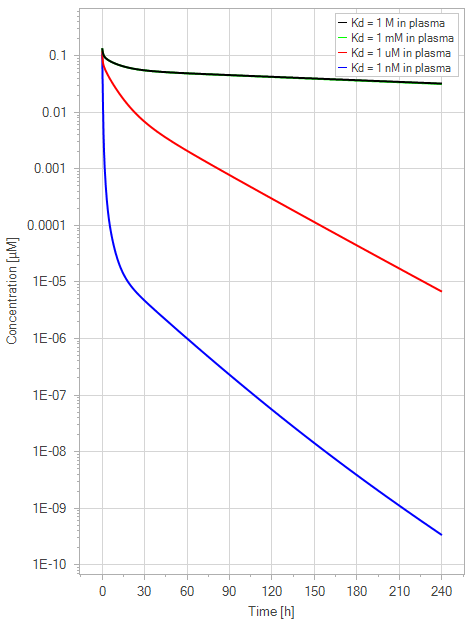
\includegraphics[width=0.49\linewidth]{pl6}
    \caption{The ``\textit{Extended Model}'' response for FcRn binding antibodies. The different line colors correspond to different FcRn affinities in plasma. The $1$ M and $1$ mM lines are overlapping. The endosomal FcRn affinity and all other parameters are kept constant at the default parameters as in Figure~\ref{fig:3} with $1$ mg/kg dose. This figure corresponds to figure 5 in the primary article.}
    \label{fig:4}
\end{figure}


\subsection{Net Model for Tg32 Mice (figure 6 in primary article)}\label{Figure6}

In order to adjust the values of the model parameters from WT to Tg32 mice, the free FcRn concentration and the endogenous IgG FcRn affinity in the endosome were modified to $95.4$ \si{\micro M} and $1$ M, respectively (see Section~\ref{MC}). To assess the effect of these alterations on the parameter values, simulations of the standard WT and Tg32 parameter sets were compared in both the net model (Figure~\ref{fig:5}) and the extended model (Figure~\ref{fig:6}).

\begin{figure}[htb]\centering
    \begin{subfigure}{0.49\textwidth}
        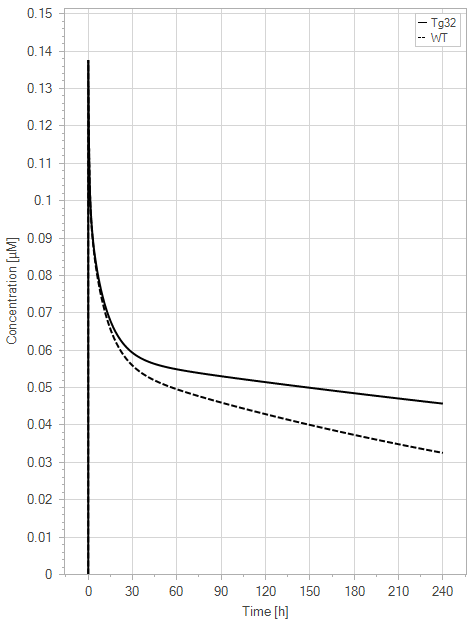
\includegraphics[width=\textwidth]{pl7.png}
        \caption{PK profiles}
        \label{fig:5a}
    \end{subfigure}
    \hfill
    \begin{subfigure}{0.49\textwidth}
        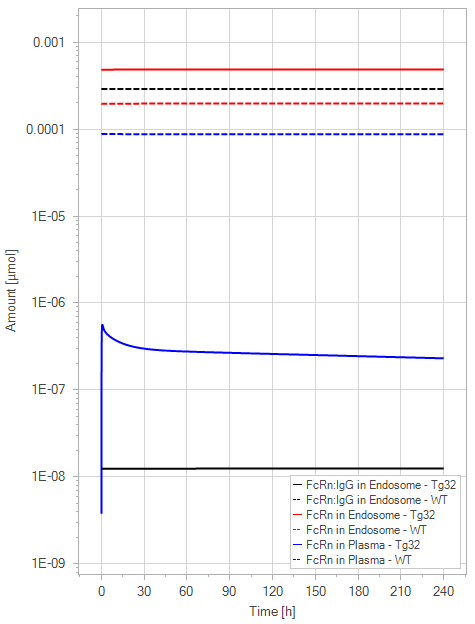
\includegraphics[width=\textwidth]{pl8.png}
        \caption{PD Profiles}
        \label{fig:5b}
    \end{subfigure}
    \caption{The ``\textit{Net Model}''response for $1$ mg/kg dose in mice with WT (dashed) and Tg32 (solid) parameter values. (a) Lines correspond to drug plasma concentrations. (b) Lines corresponds to free FcRn amounts in plasma (blue), free FcRn amounts in endosome (red) and FcRn:endogenous IgG complexes amounts in endosome (black). This figure corresponds to figure 6 in the primary article.}
    \label{fig:5}
\end{figure}

\subsubsection{Load the model}
Open the ``Physiome.mbp3'' file using MoBi\textsuperscript{\textregistered} and double-click on the ``\textit{Net Model}'' entry in the ``Simulations'' explorer.

\subsubsection{Set the Simulation for WT mice}
\begin{itemize}
    \item In the ``Parameters'' tab of our simulation, click on ``Favorites''.
    \item Change the value of the parameter: 
    \begin{itemize}
        \item \textit{DosePerBodyWeight} --> $1$ mg/kg.
    \end{itemize}
    \item ``Run'' the simulation.
    \item Rename the result in the ``Simulations'' explorer under the ``\textit{Net Model}'' entry to ``WT''.
\end{itemize}

\subsubsection{Set the Simulation for Tg32 mice}
\begin{itemize}
    \item In the ``Parameters'' tab of our simulation, click on ``Favorites''.
    \item Change the value of the parameter: 
    \begin{itemize}
        \item \textit{Start concentration of free FcRn (endosome)} --> $95.4$ \si{\micro M}
        \item \textit{EndogenousIgG | Kd (FcRn, endogenous IgG) in endosomal space} --> $1$ M
        \item \textit{EndogenousIgG | Kd (FcRn, endogenous IgG) in plasma/interstitial} --> $1$ M
    \end{itemize}
    \item ``Run'' the simulation.
    \item Rename the result in the ``Simulations'' explorer under the ``\textit{Net Model}'' entry to ``Tg32''.
\end{itemize}

\subsubsection{Compare the Results}
\begin{itemize}
    \item Double-click ``WT'' in the simulation results.
    \item Drag \& drop ``Tg32'' result onto the plot (We make it visible later).
    \item In the ``Chart Editor'', select only the ``Drug'' simulations.
    \item Make sure the Y-axis scaling is ``Linear'' in the tab ``Curves and Axis Options''.
    \item Change the ``Curve Name'' in the tab "Curves and Axis Options''.
    \begin{itemize}
        \item \textit{Tg32-Organism-PeripheralVenousBlood-Drug-Plasma (Peripheral Venous Blood)} --> Tg32
        \item \textit{WT-Organism-PeripheralVenousBlood-Drug-Plasma (Peripheral Venous Blood)} --> WT
    \end{itemize}
    \item Adjust the colors and change the title and legend position in the tab ``Chart Options''.
    \item You can find the results in Figure~\ref{fig:5}\subref{fig:5a}.
    \item Double-click ``WT'' in the simulation results again.
    \item Drag \& drop ``Tg32'' result onto the plot (We make it visible later).
    \item In the ``Chart Editor'', select only the ``FcRn'' and ``LigandEndo\_Complex'' simulations.
    \item Make sure the Y-axis scaling is ``Log'' in the tab ``Curves and Axis Options''.
    \item Change the ``Curve Name'' in the tab "Curves and Axis Options''.
    \begin{itemize}
        \item \textit{Tg32-Organism-EndogenousIgG-Endosome-LigandEndo\_Complex-Amount in container} 
        \\--> FcRn:IgG in Endosome - Tg32
        \item \textit{WT-Organism-EndogenousIgG-Endosome-LigandEndo\_Complex-Amount in container} 
        \\--> FcRn:IgG in Endosome - WT
        \item \textit{Tg32-Organism-EndogenousIgG-Endosome-FcRn-Amount in container} 
        \\--> FcRn in Endosome - Tg32
        \item \textit{WT-Organism-EndogenousIgG-Endosome-FcRn-Amount in container} 
        \\--> FcRn in Endosome - WT
        \item \textit{Tg32-Organism-EndogenousIgG-Plasma-FcRn-Amount in container} 
        \\--> FcRn in Plasma - Tg32
        \item \textit{WT-Organism-EndogenousIgG-Plasma-FcRn-Amount in container} 
        \\--> FcRn in Plasma - WT
    \end{itemize}
    \item Adjust the colors and change the title and legend position in the tab ``Chart Options''.
    \item You can find the results in Figure~\ref{fig:5}\subref{fig:5b}.
\end{itemize}

The net model showed that the lack of endogenous IgG binding caused a dramatic decrease in the amount of unbound FcRn in the plasma space (>$10,000$-fold) in comparison to the simulations of the WT. It is noteworthy that the plasma FcRn initialization was very low and was dependent on the dosage of IgG.



\subsection{Extended Model for Tg32 Mice (figure 7 in primary article)}\label{Figure7}

In the extended model, only a slight decrease in unbound FcRn is seen. For an antibody without FcRn binding in the plasma, both models demonstrate a similar contrast in PK profiles between WT and Tg32 mice. It is noteworthy that the initial plasma FcRn amount is very low, but quickly returns to its usual level.

\subsubsection{Load the model}
Open the ``Physiome.mbp3'' file using MoBi\textsuperscript{\textregistered} and double-click on the ``\textit{Extended Model}'' entry in the ``Simulations'' explorer. The steps that follow are the same as those outlined in Section~\ref{Figure6}, and the outcomes can be seen in Figure~\ref{fig:6}.

\begin{figure}[htb]\centering
    \begin{subfigure}{0.49\textwidth}
        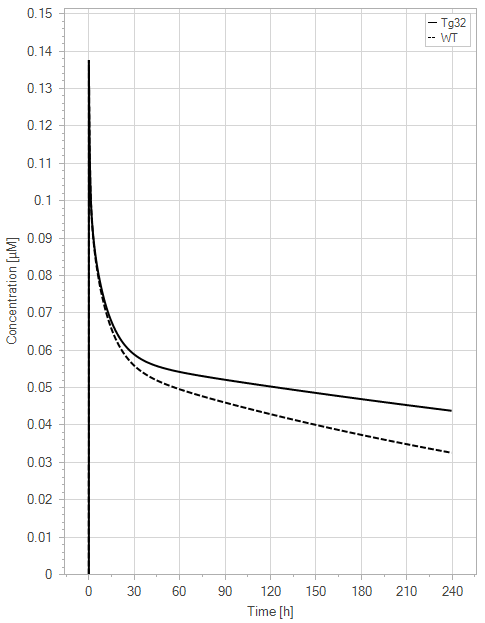
\includegraphics[width=\textwidth]{pl9.png}
        \caption{PK profiles}
        \label{fig:6a}
    \end{subfigure}
    \hfill
    \begin{subfigure}{0.49\textwidth}
        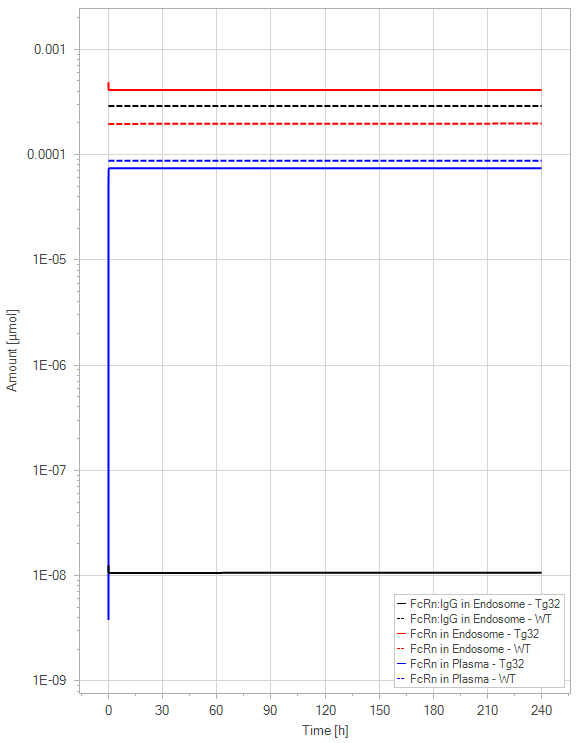
\includegraphics[width=\textwidth]{pl10.png}
        \caption{PD Profiles}
        \label{fig:6b}
    \end{subfigure}
    \caption{The ``\textit{Extended Model}''response for $1$ mg/kg dose in mice with WT (dashed) and Tg32 (solid) parameter values. (a) Lines correspond to drug plasma concentrations. (b) Lines corresponds to free FcRn amounts in plasma (blue), free FcRn amounts in endosome (red) and FcRn:endogenous IgG complexes amounts in endosome (black). This figure corresponds to figure 7 in the primary article.}
    \label{fig:6}
\end{figure}



\subsection{Extended Model YDQY for Tg32 Mice (figure 8 in primary article)}\label{Figure8}

To assess the usefulness of the extended model for molecules that bind to FcRn in the plasma, the model was tested with an experimental proof-of-concept dataset. This dataset examined the distribution of a tracer IgG after the administration of an FcRn inhibitor (YDQY) to Tg32 mice.

\subsubsection{Load the model}
Open the ``Physiome.mbp3'' file using MoBi\textsuperscript{\textregistered} and double-click on the ``\textit{Extended Model YDQY}'' entry in the ``Simulations'' explorer.

\subsubsection{Set the Simulation for Tg32 - 0 mg/kg YDQY}
\begin{itemize}
    \item In the ``Parameters'' tab of our simulation, click on ``Favorites''.
    \item Change the value of the parameter: 
    \begin{itemize}
        \item \textit{IV\_YDQY\_Application\_1-ProtocolSchemaItem | DosePerBodyWeight} --> $0$ mg/kg.
    \end{itemize}
    \item ``Run'' the simulation.
    \item Rename the result in the ``Simulations'' explorer under the ``\textit{YDQY Extended Model}'' entry to ``$0$ mg/kg''.
\end{itemize}

\subsubsection{Set the Simulation for Tg32 mice - 10 mg/kg YDQY}
\begin{itemize}
    \item In the ``Parameters'' tab of our simulation, click on ``Favorites''.
    \item Change the value of the parameter: 
    \begin{itemize}
        \item \textit{IV\_YDQY\_Application\_1-ProtocolSchemaItem | DosePerBodyWeight} --> $10$ mg/kg.
    \end{itemize}
    \item ``Run'' the simulation.
    \item Rename the result in the ``Simulations'' explorer under the ``\textit{YDQY Extended Model}'' entry to ``$10$ mg/kg''.
\end{itemize}

\subsubsection{Set the Simulation for Tg32 mice - 20 mg/kg YDQY}
\begin{itemize}
    \item In the ``Parameters'' tab of our simulation, click on ``Favorites''.
    \item Change the value of the parameter: 
    \begin{itemize}
        \item \textit{IV\_YDQY\_Application\_1-ProtocolSchemaItem | DosePerBodyWeight} --> $20$ mg/kg.
    \end{itemize}
    \item ``Run'' the simulation.
    \item Rename the result in the ``Simulations'' explorer under the ``\textit{YDQY Extended Model}'' entry to ``$20$ mg/kg''.
\end{itemize}

\subsubsection{Set the Simulation for Tg32 mice - 3x20 mg/kg YDQY}
\begin{itemize}
    \item In the ``Parameters'' tab of our simulation, click on ``Favorites''.
    \item Change the value of the parameter: 
    \begin{itemize}
        \item \textit{IV\_YDQY\_Application\_1-ProtocolSchemaItem | DosePerBodyWeight} --> $20$ mg/kg.
        \item \textit{IV\_YDQY\_Application\_2-ProtocolSchemaItem | DosePerBodyWeight} --> $20$ mg/kg.
        \item \textit{IV\_YDQY\_Application\_3-ProtocolSchemaItem | DosePerBodyWeight} --> $20$ mg/kg.
    \end{itemize}
    \item ``Run'' the simulation.
    \item Rename the result in the ``Simulations'' explorer under the ``\textit{YDQY Extended Model}'' entry to ``$3x20$ mg/kg''.
\end{itemize}

\subsubsection{Set the Simulation for Tg32 mice - 40 mg/kg YDQY}
\begin{itemize}
    \item In the ``Parameters'' tab of our simulation, click on ``Favorites''.
    \item Change the value of the parameter: 
    \begin{itemize}
        \item \textit{IV\_YDQY\_Application\_1-ProtocolSchemaItem | DosePerBodyWeight} --> $40$ mg/kg.
        \item \textit{IV\_YDQY\_Application\_2-ProtocolSchemaItem | DosePerBodyWeight} --> $0$ mg/kg.
        \item \textit{IV\_YDQY\_Application\_3-ProtocolSchemaItem | DosePerBodyWeight} --> $0$ mg/kg.
    \end{itemize}
    \item ``Run'' the simulation.
    \item Rename the result in the ``Simulations'' explorer under the ``\textit{YDQY Extended Model}'' entry to ``$40$ mg/kg''.
\end{itemize}

\subsubsection{Compare Results}
The observed data is imported and can be found in the "Building Blocks" explorer under the "Observed Data" section.
\begin{itemize}
    \item Double-click ``$0$ mg/kg'' in the simulation results.
    \item Expand ``Observed Data'' and drag \& drop ``hIgG'' onto the simulation results chart.
    \item In the ``Chart Editor'', select only the ``hIgG'' simulations.
    \item Make sure the Y axis scaling is ``Log'' in the tab ``Curves and Axis Options''.
    \item Change the ``Curve Name'' in the tab "Curves and Axis Options''.
    \begin{itemize}
        \item \textit{0 mg/kg-Organism-PeripheralVenousBlood-hIgG-Plasma (Peripheral Venous Blood)} 
        \\--> hIgG - Simulation
        \item \textit{hIgG-hIgG-Measurement} --> hIgG - Measurement
    \end{itemize}
    \item Adjust the colors and change the title and legend position in the tab ``Chart Options''.
    \item You can find the results in Figure~\ref{fig:7}\subref{fig:7a}.
    \item Double-click ``$10$ mg/kg'' in the simulation results.
    \item Expand ``Observed Data'' and drag \& drop ``hIgG+10.YDQY'' and ``10.YDQY'' onto the simulation results chart.
    \item In the ``Chart Editor'', select only the ``hIgG'' and ``YDQY'' simulations.
    \item Make sure the Y axis scaling is ``Log'' in the tab ``Curves and Axis Options''.
    \item Change the ``Curve Name'' in the tab "Curves and Axis Options''.
    \begin{itemize}
        \item \textit{10 mg/kg-Organism-PeripheralVenousBlood-hIgG-Plasma (Peripheral Venous Blood)} 
        \\--> hIgG -  Simulation
        \item \textit{hIgG+10.YDQY-hIgG+10.YDQY-Measurement} --> hIgG - Measurement
        \item \textit{10 mg/kg-Organism-PeripheralVenousBlood-YDQY-Plasma (Peripheral Venous Blood)} --> YDQY - Simulation
        \item \textit{10.YDQY-10.YDQY-Measurement} --> YDQY - Measurement
    \end{itemize}
    \item Adjust the colors and change the title and legend position in the tab ``Chart Options''.
    \item You can find the results in Figure~\ref{fig:7}\subref{fig:7b}.
    \item Double-click ``$20$ mg/kg'' in the simulation results.
    \item Expand ``Observed Data'' and drag \& drop ``hIgG+20.YDQY'' and ``20.YDQY'' onto the simulation results chart.
    \item In the ``Chart Editor'', select only the ``hIgG'' and ``YDQY'' simulations.
    \item Make sure the Y axis scaling is ``Log'' in the tab ``Curves and Axis Options''.
    \item Change the ``Curve Name'' in the tab "Curves and Axis Options''.
    \begin{itemize}
        \item \textit{20 mg/kg-Organism-PeripheralVenousBlood-hIgG-Plasma (Peripheral Venous Blood)} 
        \\--> hIgG -  Simulation
        \item \textit{hIgG+20.YDQY-hIgG+20.YDQY-Measurement} --> hIgG - Measurement
        \item \textit{20 mg/kg-Organism-PeripheralVenousBlood-YDQY-Plasma (Peripheral Venous Blood)} --> YDQY - Simulation
        \item \textit{20.YDQY-20.YDQY-Measurement} --> YDQY - Measurement
    \end{itemize}
    \item Adjust the colors and change the title and legend position in the tab ``Chart Options''.
    \item You can find the results in Figure~\ref{fig:7}\subref{fig:7c}.
    \item Double-click ``$3x20$ mg/kg'' in the simulation results.
    \item Expand ``Observed Data'' and drag \& drop ``hIgG+3x20.YDQY'' and ``3x20.YDQY'' onto the simulation results chart.
    \item In the ``Chart Editor'', select only the ``hIgG'' and ``YDQY'' simulations.
    \item Make sure the Y axis scaling is ``Log'' in the tab ``Curves and Axis Options''.
    \item Change the ``Curve Name'' in the tab "Curves and Axis Options''.
    \begin{itemize}
        \item \textit{3x20 mg/kg-Organism-PeripheralVenousBlood-hIgG-Plasma (Peripheral Venous Blood)} 
        \\--> hIgG -  Simulation
        \item \textit{hIgG+3x20.YDQY-hIgG+3x20.YDQY-Measurement} --> hIgG - Measurement
        \item \textit{3x20 mg/kg-Organism-PeripheralVenousBlood-YDQY-Plasma (Peripheral Venous Blood)} --> YDQY - Simulation
        \item \textit{3x20.YDQY-3x20.YDQY-Measurement} --> YDQY - Measurement
    \end{itemize}
    \item Adjust the colors and change the title and legend position in the tab ``Chart Options''.
    \item You can find the results in Figure~\ref{fig:7}\subref{fig:7d}.
    \item Double-click ``$40$ mg/kg'' in the simulation results.
    \item Expand ``Observed Data'' and drag \& drop ``hIgG+40.YDQY'' and ``40.YDQY'' onto the simulation results chart.
    \item In the ``Chart Editor'', select only the ``hIgG'' and ``YDQY'' simulations.
    \item Make sure the Y axis scaling is ``Log'' in the tab ``Curves and Axis Options''.
    \item Change the ``Curve Name'' in the tab "Curves and Axis Options''.
    \begin{itemize}
        \item \textit{40 mg/kg-Organism-PeripheralVenousBlood-hIgG-Plasma (Peripheral Venous Blood)} 
        \\--> hIgG -  Simulation
        \item \textit{hIgG+40.YDQY-hIgG+40.YDQY-Measurement} --> hIgG - Measurement
        \item \textit{40 mg/kg-Organism-PeripheralVenousBlood-YDQY-Plasma (Peripheral Venous Blood)} --> YDQY - Simulation
        \item \textit{40.YDQY-40.YDQY-Measurement} --> YDQY - Measurement
    \end{itemize}
    \item Adjust the colors and change the title and legend position in the tab ``Chart Options''.
    \item You can find the results in Figure~\ref{fig:7}\subref{fig:7e}.
\end{itemize}

The extended model was capable of representing the PK profile of both WT IgG and YDQY, as well as the effect of YDQY dosing on the concentration of wild-type IgG, as illustrated in Figure~\ref{fig:7}.

\begin{figure}[htb]\centering
    \begin{subfigure}{0.32\textwidth}
        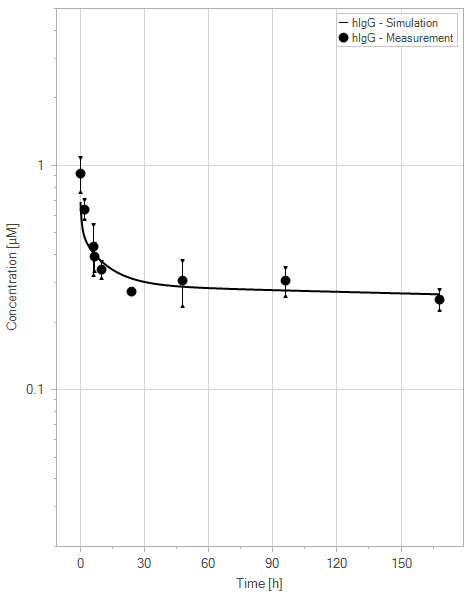
\includegraphics[width=\textwidth]{pl11.png}
        \caption{hIgG = 0 mg/kg}
        \label{fig:7a}
    \end{subfigure}
    \hfill
    \begin{subfigure}{0.32\textwidth}
        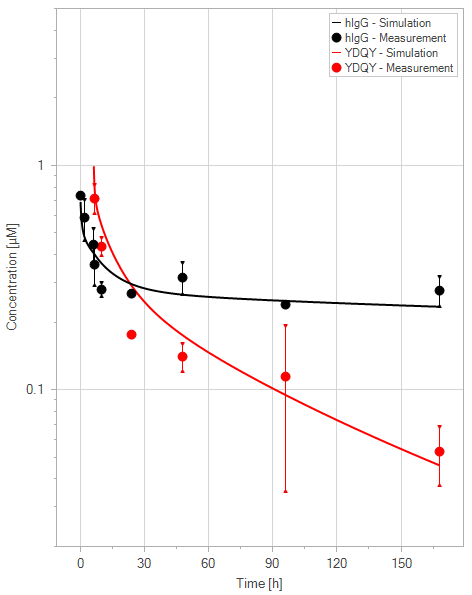
\includegraphics[width=\textwidth]{pl12.png}
        \caption{YDQY = 10 mg/kg}
        \label{fig:7b}
    \end{subfigure}
    \hfill
    \begin{subfigure}{0.32\textwidth}
        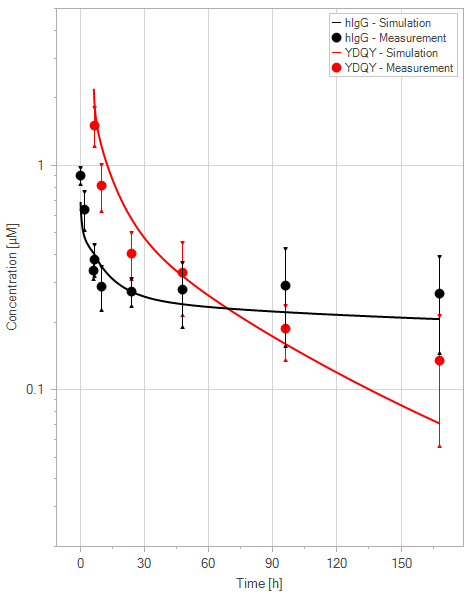
\includegraphics[width=\textwidth]{pl13.png}
        \caption{YDQY = 20 mg/kg}
        \label{fig:7c}
    \end{subfigure}
    \hfill
    \begin{subfigure}{0.32\textwidth}
        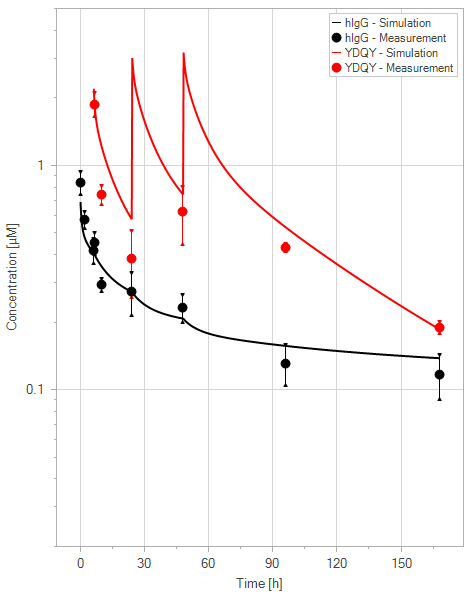
\includegraphics[width=\textwidth]{pl14.png}
        \caption{YDQY = 3x20 mg/kg}
        \label{fig:7d}
    \end{subfigure}
    \hfill
    \begin{subfigure}{0.32\textwidth}
        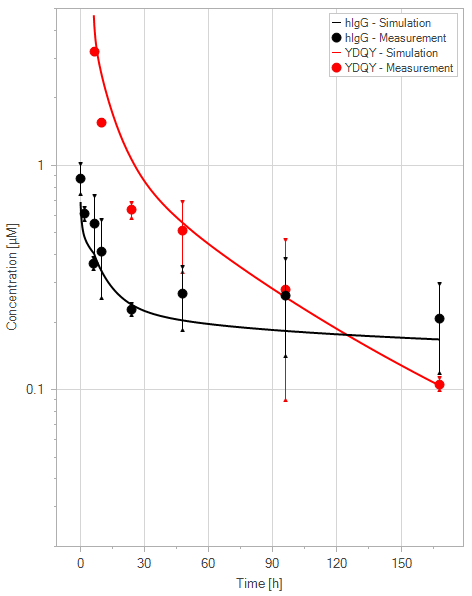
\includegraphics[width=\textwidth]{pl15.png}
        \caption{YDQY = 40 mg/kg}
        \label{fig:7e}
    \end{subfigure}
    \caption{Fit of hIgG (black) and YDQY (red) plasma concentrations for different dosing scenarios (a-e). Lines are the model predictions, and dots are observed mean plasma concentration data with error bars indicating the standard deviations. This figure corresponds to figure 8 in the primary article.}
    \label{fig:7}
\end{figure}

%-------------------------------------------------------------------
%-------------------------------------------------------------------
%-------------------------------------------------------------------

\section{Discussion}

In this article, we introduced a mechanistic model of FcRn-mediated recycling of large molecules, which was initially proposed by \cite{de2023mechanistic}, using MoBi\textsuperscript{\textregistered}. Our implementation is modular and can be adapted to various coupling scenarios without having to modify the main model. The figures from the original publication were accurately reproduced, with only minor changes to the legends. 

%-------------------------------------------------------------------
%-------------------------------------------------------------------
%-------------------------------------------------------------------

\section{Conclusion}

In conclusion, the extended model proposed by \cite{de2023mechanistic} has proven to be useful for FcRn inhibitors in the plasma environment. Although further refinement of the model is necessary to validate and correlate the parameter values, the current version of the extended model already offers the ability to adjust the plasma half-life in relation to the FcRn affinity in plasma, which was not available in the original model. We have also outlined all the input parameters in Tables~\ref{tbl:2},~\ref{tbl:3},~\ref{tbl:4} for Net and Extended models to guide conducting appropriate in vitro and in vivo experiments. These experiments will be able to generate key model parameters for meaningful simulations to inform construct engineering, interspecies translation and/or dose selection.

\begin{landscape}
\begin{table}[htbp]
\centering
    \begin{threeparttable}
        \caption{List of all the input parameters for the Net model.}\label{tbl:2}
        \begin{tabular}{ccclcl}
            \toprule
            Top Container & Container & Molecule & Name & Value & Unit\\
            \midrule
            Organism & - & - & Rate constant for endosmal uptake (global) & $0.29$ & 1/min \\
            Organism & - & - & Rate constant for recycling from endosomal space (global) & $0.09$ & 1/min \\
            Organism & - & - & Specific clearance (endosome) & $0.21$ & 1/min \\
            Organism & Endogenous IgG & - & Kd (FcRn, endogenous IgG) in endosomal space & $0.75$ & \si{\micro M} \\
            Organism & Endogenous IgG & - & Kd (FcRn, endogenous IgG) in plasma/interstitial & $10000$ & \si{\micro M} \\
            Organism & Endogenous IgG & Endosome & Start concentration of free FcRn (endosome) & $38.7$ & \si{\micro M} \\
            - & - & Drug & Is small molecule & $0$ & -\\
            - & - & Drug & Molecular weight & $150000$ & g/mol\\
            - & - & Drug & Plasma protein binding partner & $1.0$ & -\\
            - & - & Drug & Lipophilicity & $-5$ & Log Units \\
            - & - & Drug & Fraction unbound (plasma) & $1.0$ & - \\
            - & - & Drug & Solubility & $10000$ & mg/l\\
            - & - & Drug & Reference pH & $7.0$ & -\\
            - & - & Drug & Kd (FcRn) in endosomal space & $1.0$ & \si{\micro M}\\
            - & - & Drug & Kd (FcRn) in plasma/interstitial & $1.0$ & M\\
            Applications & IV-Drug-Application\_1 & - & Start time & $0.0$ & h \\
            Applications & IV-Drug-Application\_1 & - & DosePerBodyWeight & $1.0$ & mg/kg \\
            \bottomrule
        \end{tabular}
    \end{threeparttable}
\end{table}
\end{landscape}

\begin{landscape}
\begin{table}[htbp]
\centering
    \begin{threeparttable}
        \caption{List of all the input parameters for the Extended model.}\label{tbl:3}
        \begin{tabular}{ccclcl}
            \toprule
            Top Container & Container & Molecule & Name & Value & Unit \\
            \midrule
            Organism & - & - & Rate constant for endosmal uptake (global) & $0.49$ & 1/min \\
            Organism & - & - & Rate constant for recycling from endosomal space (global) & $0.09$ & 1/min \\
            Organism & - & - & Specific clearance (endosome) & $0.21$ & 1/min \\
            Organism & Endogenous IgG & - & Krpls & $1.45$e-4 & l/min \\
            Organism & Endogenous IgG & - & IgG\_kpe & $1.50$e-6 & l/min \\
            Organism & Endogenous IgG & - & Kd (FcRn, endogenous IgG) in endosomal space & $0.75$ & \si{\micro M} \\
            Organism & Endogenous IgG & - & Kd (FcRn, endogenous IgG) in plasma/interstitial & $10000$ & \si{\micro M} \\
            Organism & Endogenous IgG & Endosome & Start concentration of free FcRn (endosome) & $38.7$ & \si{\micro M} \\
            - & - & Drug & Is small molecule & $0$ &-\\
            - & - & Drug & Molecular weight & $150000$ & g/mol\\
            - & - & Drug & Plasma protein binding partner & $1.0$ &-\\
            - & - & Drug & Lipophilicity & $-5$ & Log Units \\
            - & - & Drug & Fraction unbound (plasma) & $1.0$ &-\\
            - & - & Drug & Solubility & $10000$ & mg/l\\
            - & - & Drug & Reference pH & $7.0$ &-\\
            - & - & Drug & Kd (FcRn) in endosomal space & $1.0$ & \si{\micro M}\\
            - & - & Drug & Kd (FcRn) in plasma/interstitial & $1.0$ & M\\
            Applications & IV-Drug-Application\_1 & - & Start time & $0.0$ & h \\
            Applications & IV-Drug-Application\_1 & - & DosePerBodyWeight & $1.0$ & mg/kg \\
            \bottomrule
        \end{tabular}
    \end{threeparttable}
\end{table}
\end{landscape}

\begin{landscape}
\begin{table}[htbp]
\centering
    \begin{threeparttable}
        \caption{List of all the input parameters for the Extended model YDQY.}\label{tbl:4}
        \begin{tabular}{ccclcl}
            \toprule
            Top Container & Container & Molecule & Name & Value & Unit \\
            \midrule
            Organism & - & - & Rate constant for endosmal uptake (global) & $0.49$ & 1/min \\
            Organism & - & - & Rate constant for recycling from endosomal space (global) & $0.09$ & 1/min \\
            Organism & - & - & Specific clearance (endosome) & $0.21$ & 1/min \\
            Organism & Endogenous IgG & - & Krpls & $1.45$e-4 & l/min \\
            Organism & Endogenous IgG & - & IgG\_kpe & $1.50$e-6 & l/min \\
            Organism & Endogenous IgG & - & Kd (FcRn, endogenous IgG) in endosomal space & $1000000$ & \si{\micro M} \\
            Organism & Endogenous IgG & - & Kd (FcRn, endogenous IgG) in plasma/interstitial & $1000000$ & \si{\micro M} \\
            Organism & Endogenous IgG & Endosome & Start concentration of free FcRn (endosome) & $95.4$ & \si{\micro M} \\
            - & - & hIgG & Is small molecule & $0$ & -\\
            - & - & hIgG & Molecular weight & $150000$ & g/mol\\
            - & - & hIgG & Plasma protein binding partner & $1.0$ & -\\
            - & - & hIgG & Lipophilicity & $-5$ & Log Units \\
            - & - & hIgG & Fraction unbound (plasma) & $1.0$ & -\\
            - & - & hIgG & Solubility & $10000$ & mg/l\\
            - & - & hIgG & Reference pH & $7$ & -\\
            - & - & hIgG & Kd (FcRn) in endosomal space & $0.4$ & \si{\micro M}\\
            - & - & hIgG & Kd (FcRn) in plasma/interstitial & $1000000$ & \si{\micro M}\\
            Applications & IV-hIgG-Application\_1 & - & Start time & $0.0$ & h \\
            Applications & IV-hIgG-Application\_1 & - & DosePerBodyWeight & $5.0$ & mg/kg \\
            - & - & YDQY & Is small molecule & $0$ & -\\
            - & - & YDQY & Molecular weight & $150000$ & g/mol\\
            - & - & YDQY & Plasma protein binding partner & $1.0$ & -\\
            - & - & YDQY & Lipophilicity & $-5$ & Log Units \\
            - & - & YDQY & Fraction unbound (plasma) & $1.0$ & -\\
            - & - & YDQY & Solubility & $10000$ & mg/l\\
            - & - & YDQY & Reference pH & $7$ & -\\
            - & - & YDQY & Kd (FcRn) in endosomal space & $0.08$ & \si{\micro M}\\
            - & - & YDQY & Kd (FcRn) in plasma/interstitial & $0.12$ & \si{\micro M}\\
            Applications & IV-YDQY-Application\_1 & - & Start time & $6.0$ & h \\
            Applications & IV-YDQY-Application\_1 & - & DosePerBodyWeight & $10.0$ & mg/kg \\
            Applications & IV-YDQY-Application\_2 & - & Start time & $24.0$ & h \\
            Applications & IV-YDQY-Application\_2 & - & DosePerBodyWeight & $0.0$ & mg/kg \\
            Applications & IV-YDQY-Application\_3 & - & Start time & $48.0$ & h \\
            Applications & IV-YDQY-Application\_3 & - & DosePerBodyWeight & $0.0$ & mg/kg \\
            \bottomrule
        \end{tabular}
    \end{threeparttable}
\end{table}
\end{landscape}

\section{Acknowledgement}

SS, VDB, LBA, TVB and MLS are employees of Sanofi and may hold shares and/or stock options in the company.

\bibliography{sample}

\end{document}